\section{Relationship Modeling}\label{sec:relationship_modeling}

\subsection{Component, Spanner, Indicator}

Some text here.

\subsection{Hierarchical relationships}

\begin{lstlisting}
>>> staff = Staff()
>>> outer_tuplet_one = Tuplet((2, 3), "d''16 ef'8.")
>>> inner_tuplet = Tuplet((4, 5), "cs''16 e'16 d'2")
>>> outer_tuplet_one.append(inner_tuplet)
>>> outer_tuplet_two = Tuplet((4, 5), "d'8 r16 b'16 as'16")
>>> staff.extend([outer_tuplet_one, outer_tuplet_two])
>>> staff.extend("as'8.. fs'32")
>>> show(staff)
\end{lstlisting}

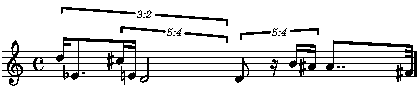
\includegraphics[scale=1.0]{images/section_4_relationship_modeling-1.pdf}


Abjad provides concrete object-models for various hierarchical relationships

Parentage, Lineage, Leaves

\begin{lstlisting}
>>> staff_leaves = staff.select_leaves()
>>> for leaf in staff_leaves:
...     leaf
... 
Note("d''16")
Note("ef'8.")
Note("cs''16")
Note("e'16")
Note("d'2")
Note("d'8")
Rest('r16')
Note("b'16")
Note("as'16")
Note("as'8..")
Note("fs'32")
\end{lstlisting}


\begin{lstlisting}
>>> tuplet_leaves = outer_tuplet_one.select_leaves()
>>> for leaf in tuplet_leaves:
...     leaf
... 
Note("d''16")
Note("ef'8.")
Note("cs''16")
Note("e'16")
Note("d'2")
\end{lstlisting}


\begin{lstlisting}
>>> third_note = staff_leaves[2]
>>> third_note
Note("cs''16")
\end{lstlisting}



\begin{lstlisting}
>>> parentage = inspect_(third_note).get_parentage()
>>> parentage.root
<Staff{4}>
\end{lstlisting}


\begin{lstlisting}
>>> parentage.tuplet_depth
2
\end{lstlisting}


\begin{lstlisting}
>>> parentage.prolation
Multiplier(8, 15)
\end{lstlisting}


Selections

Bidirectional vs unidirectional pointers.

\subsection{Attachment relationships}

\begin{lstlisting}
>>> leaves = staff.select_leaves()
>>> attach(Tie(), leaves[4:6])
>>> attach(Tie(), leaves[-3:-1])
>>> attach(Slur(), leaves[:2])
>>> attach(Slur(), leaves[2:6])
>>> final_slur = Slur()
>>> attach(final_slur, leaves[7:])
>>> attach(Dynamic('f'), leaves[0])
>>> attach(Dynamic('p'), leaves[-4])
>>> attach(Articulation('accent'), leaves[0])
>>> attach(Articulation('accent'), leaves[2])
>>> show(staff)
\end{lstlisting}

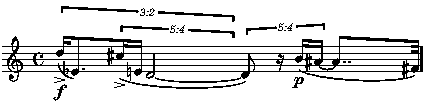
\includegraphics[scale=1.0]{images/section_4_relationship_modeling-2.pdf}


\begin{lstlisting}
>>> spanners = inspect_(leaves[0]).get_spanners(Slur)
>>> first_slur = tuple(spanners)[0]
>>> first_slur.components
Selection(Note("d''16"), Note("ef'8."))
\end{lstlisting}


\begin{lstlisting}
>>> for leaf in leaves:
...     dynamic = inspect_(leaf).get_effective(Dynamic)
...     print(dynamic, leaf)
... 
Dynamic(name='f') d''16
Dynamic(name='f') ef'8.
Dynamic(name='f') cs''16
Dynamic(name='f') e'16
Dynamic(name='f') d'2
Dynamic(name='f') d'8
Dynamic(name='f') r16
Dynamic(name='p') b'16
Dynamic(name='p') as'16
Dynamic(name='p') as'8..
Dynamic(name='p') fs'32
\end{lstlisting}


Spanners.

Indicator scope.

\subsection{Temporal relationships}

Logical ties.

\begin{lstlisting}
>>> for logical_tie in iterate(staff).by_logical_tie():
...     logical_tie
... 
LogicalTie(Note("d''16"),)
LogicalTie(Note("ef'8."),)
LogicalTie(Note("cs''16"),)
LogicalTie(Note("e'16"),)
LogicalTie(Note("d'2"), Note("d'8"))
LogicalTie(Rest('r16'),)
LogicalTie(Note("b'16"),)
LogicalTie(Note("as'16"), Note("as'8.."))
LogicalTie(Note("fs'32"),)
\end{lstlisting}

